\section {Experimental Part}



The Revisited Box Counting technique will be tested on models of deterministic self-similar 2D fractal sets. They are generated by recursive expansion of binary matrix $\mathbb{G}_{u,v} \in \{ 0, 1 \}^{v \times v} $, where $u$ a is the number of non-zero elements (units), $v>1$ is a matrix dimension, and $v<u<v^2$. \\
\\*
Recursive expansion of $\mathbb{G}_{u,v}$ generates a binary matrix which represents fractal set $\mathbb{F}_{u,v}$ of a similarity dimension $D_{\text{S}} = D_{\text{H}} = D_{0} = D_{1} = \frac{\log{u}}{\log{v}}$. Depth $h$ of recursion depends on $v$ and should be appropriate to computer memory size. The structures involved in the research are depicted in Fig. \ref{fig:involvedFractals}\\
\\*
\begin{figure}[tbp]
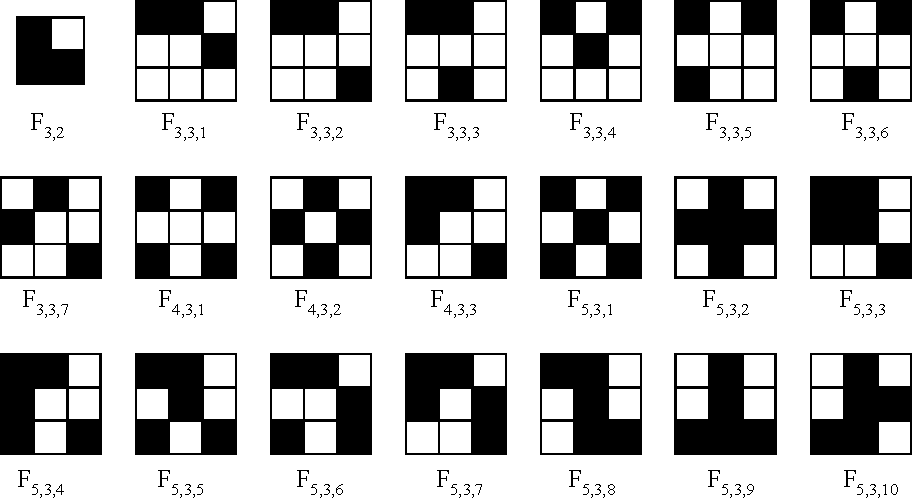
\includegraphics[width=\textwidth]{images/fractals.pdf} 
\caption{Table of the fractals involved in the research}
\label{fig:involvedFractals}
\end{figure}
At first, adequate point sets of given depth $h$ were generated. Then, they were randomly rotated around the origin, and finally they were randomly shifted. Afterwards, a grid of size $a$ was put on the data points and entropy estimates were calculated. Due to physical interpretation of entropy, the estimates were averaged over 20 realizations and mean values of entropy were calculated. \\
\\*
The relationship between $\hat{D}_{\mathrm{naive}}$ and optimum value of $\alpha$ was studied on the aforementioned fractals for the grid of size $a=12,16,20,...,480,500$.  The results of optimization are collected in Tab. \ref{tab:table1}. We suppose, the relationship can be approximated by linear, exponential, or power model respectively as
\begin{equation}
\label{eq:models}
\begin{split}
 \alpha &= A + B \hat{D}_{0,\mathrm{naive}}, \\
 \ln \alpha &= A + B \hat{D}_{0,\mathrm{naive}}, \\
 \ln \alpha &= A + B \ln \hat{D}_{0,\mathrm{naive}}.
\end{split}
\end{equation}
\\*
Linear regression was used for the estimation of unknown parameters $A$ and $B$. The values are included in Tab. \ref{tab:model_results} together with correlation coefficient $r$. The exponential model had the best correlation and will be used for corrected estimation. But the differences among models are not statistically significant. Using exponential model, we calculated $\alpha_{\mathrm{model}}$ from $\hat{D}_{0,\mathrm{naive}}$, then recalculated $\hat{D}_0$, and tested hypothesis $\mathrm{H}_0:\text{E}\hat{D}_{0} = D_{0}$ via two-sided t-test. The resulting values are also collected in Tab. \ref{tab:table1} as $\hat{D}_{0}$ and $p_{\mathrm{value}}$. In this case of multiple hypothesis testing we had to apply False Discovery Rate (FDR) [\ref{bib:FDR}] methodology on critical level $p_{crit} = 0.05$. We were not able to reject any hypotheses and therefore the improved $\hat{D}_{0}$ estimate was not biased in our experiments.



\begin{figure}[tbp]
\centering
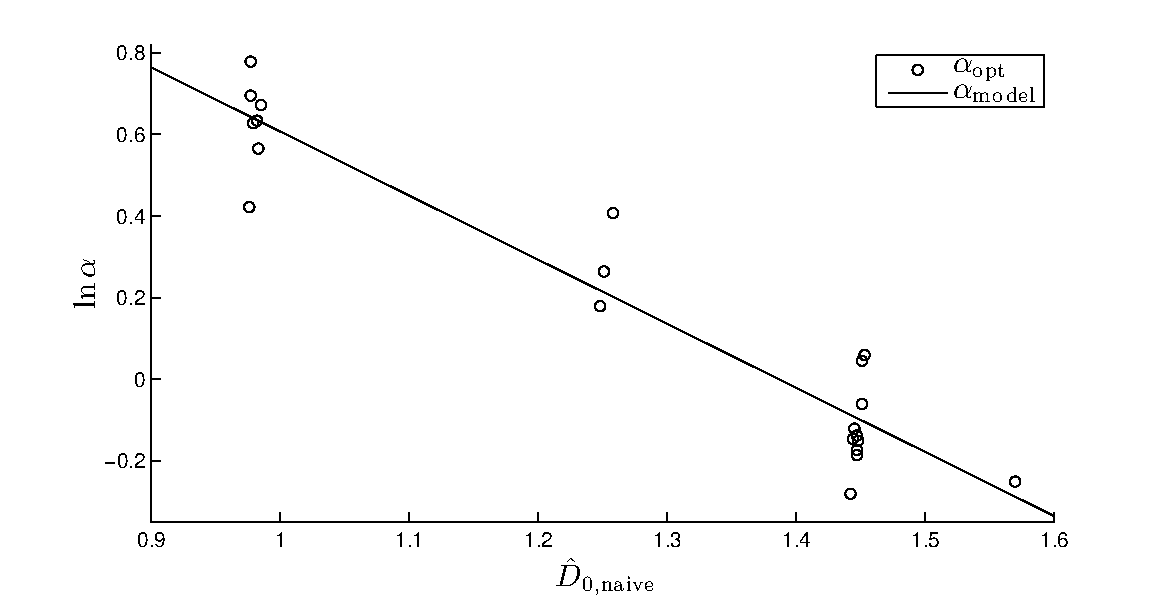
\includegraphics[scale=0.6]{images/graph_alpha_model} 
\caption{Optimum $\alpha$ values of exponential model and its linear regression}
\label{fig:graphAlphaModel}
\end{figure}

\begin{table}[tbp]
\centering
\caption{Optimum $\alpha$ values and their exponential model}
\label{tab:table1}
\begin{tabular}{|l||l|l||l|l||l|l|}
\hline
Fractal & $h$ & $D_{0}$ & $\hat{D}_{0,\mathrm{naive}}$ & $\alpha_{\mathrm{opt}}$ & $\alpha_{\mathrm{model}}$ & $p_{\mathrm{value}}$ \\ \hline \hline
$\mathrm{F_{3,2}}$ & 11 & 1.585 & 1.567 & 0.778 & 0.749 &	0.392  \\
$\mathrm{F_{3,3,1}}$ & 7 & 1 & 0.982 & 1.885 & 1.886	& 0.995 \\
$\mathrm{F_{3,3,2}}$ & 7 & 1 & 0.977 & 2.178 & 1.901	& 0.131 \\
$\mathrm{F_{3,3,3}}$ & 7 & 1 & 0.977 & 2.004 &  1.901	& 0.667  \\
$\mathrm{F_{3,3,4}}$ & 7 & 1 & 0.985 & 1.958 &  1.878	& 0.743  \\
$\mathrm{F_{3,3,5}}$ & 7 & 1 & 0.976 & 1.525 &  1.904	& 0.129  \\
$\mathrm{F_{3,3,6}}$ & 7 & 1 & 0.983 & 1.760 &  1.883	& 0.698  \\
$\mathrm{F_{3,3,7}}$ & 7 & 1 & 0.979 & 1.873 &  1.895 &	0.929  \\
$\mathrm{F_{4,3,1}}$ & 7 & 1.262 & 1.251 & 1.302 &  1.236	& 0.789  \\
$\mathrm{F_{4,3,2}}$ & 7 & 1.262 & 1.248 & 1.196 &  1.242	& 0.850  \\
$\mathrm{F_{4,3,3}}$ & 7 & 1.262 & 1.258 & 1.502 &  1.223	& 0.283  \\
$\mathrm{F_{5,3,1}}$ & 7 & 1.465 & 1.447 & 0.871 &  0.908	& 0.653  \\
$\mathrm{F_{5,3,2}}$ & 7 & 1.465 & 1.447 & 0.830 &  0.908	& 0.427  \\
$\mathrm{F_{5,3,3}}$ & 7 & 1.465 & 1.451 & 0.941 &  0.903	& 0.544  \\
$\mathrm{F_{5,3,4}}$ & 7 & 1.465 & 1.445 & 0.886 &  0.911	& 0.720  \\
$\mathrm{F_{5,3,5}}$ & 7 & 1.465 & 1.444 & 0.864 &  0.913	& 0.367  \\
$\mathrm{F_{5,3,6}}$ & 7 & 1.465 & 1.451 & 1.046 &  0.903	& 0.185  \\
$\mathrm{F_{5,3,7}}$ & 7 & 1.465 & 1.453 & 1.061 &  0.900	& 0.019  \\
$\mathrm{F_{5,3,8}}$ & 7 & 1.465 & 1.447 & 0.841 &  0.908	& 0.122  \\
$\mathrm{F_{5,3,9}}$ & 7 & 1.465 & 1.442 & 0.755 &  0.916	& 0.009  \\
$\mathrm{F_{5,3,10}}$ & 7 & 1.465 & 1.448 & 0.860 &  0.907 & 0.186  \\ \hline
\end{tabular}
\end{table}

\begin{table}[tbp]
\centering
\caption{Comparison of the models fitting the relationship between $\hat{D}_{0,\mathrm{naive}}$ and $\alpha$}
\label{tab:model_results}
\begin{tabular}{r||l|l|l}
model       & $A$ & $B$ & $r$ \\ \hline \hline
linear      & 3.905 & --2.066 & --0.9542 \\
exponential & 2.178 & --1.571 & --0.9553 \\
power       & 0.605 & --1.892 & --0.9524
\end{tabular}
\end{table}